%% Encoding: ISO8859-1 %%

\section{Allgemeines}
\subsection{Subsection 1.1}
\frame{
\frametitle{Allgemeines}
\begin{itemize}
    \item neue Art von Schaltkreis (Nanoelektronik) 
    \item Signale als Token auf Kabeln 
    \item Fluktuation der Token als treibende Kraft f�r Berechnungen
\end{itemize}
}
\subsection{Token-pass Schaltkreise}
\frame{
\frametitle{Token-pass Schaltkreise}
\begin{itemize}
    \item T-Element als Grundbauteil 
\end{itemize}

\begin{figure}
    \begin{flushright}
        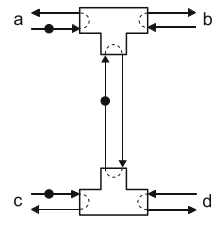
\includegraphics[height=5cm]{bilder/2-T-Elemente.png} 
    \end{flushright}
\end{figure}
}
